\chapter{Software Test Plan}
\section{Inleiding}
Het systeem kan op verschilende manieren getest worden. 
Langs de ene kant zijn er tests voor onafhankelijke stukken code (Unittests), en langs de andere kant wordt de samenwerking van deze componenten getest (Integratietests). 
Daarnaast moet op vlak van GUI getest worden of de applicatie stabiel blijft in bepaalde scenario's, of bij foute input van gebruikers. 
Door middel van tests moet gegarandeerd worden dat het systeem werkt en voldoet aan de specificaties beschreven in het SRS\cite{srs}. 
Programmeurs mogen slechts code pushen naar de hoofdrepository wanneer alle aanwezige tests nog steeds correct uitgevoerd worden.
Wanneer voldoende tests zijn geschreven voor alle relevante onderdelen garandeert dit dat het systeem werkt zoals men verwacht.

\section{Soorten tests}

\subsection{Unittests}
Unittests zijn tests die kleine, onafhankelijke stukken code testen. Code die door unittests getest wordt mag geen gebruik maken van externe bronnen, anders kan men niet nagaan of de fout in de te testen klasse/methode zit, of in de externe code.
Wanneer een klasse wordt afgewerkt (of een subset van zijn methoden) moet hiervoor reeks unittests worden geschreven. 
Deze tests moeten correctheid van een individueel component nagaan. 
Wanneer de klasse wordt aangepast kunnen eventuele nieuwe problemen worden gedetecteerd door het opnieuw runnen van de gemaakte tests. 

\subsection{Integratietests}
Integratie testing is het onderdeel van testing waar individuele componenten worden samengebracht en hun samenwerking getest.
Deze tests gebeuren conceptueel na unittesting (het testen van individuele componenten) en voor verificatietesten. 
De bedoeling van integratietesting is het verifi\"{e}ren van functionele-, performantie- en betrouwbaarheidsrequirements. 
Test cases zorgen ervoor dat een bepaalde groep van componenten correct interageren met elkaar.
Een onderdeel van integratietesten is verificatie, en zo gaat er dus geverifi\"{e}erd worden dat dat het systeem voldoet aan de requirements beschreven in het SRS\cite{srs}. 

\subsection{GUI tests}
De GUI wordt ook uitvoerig getest.
Deze moet blijven werken zoals verwacht met willekeurige input, mogelijk met kwade bedoelingen (denk aan SQL-injecties). 
De automatisering van deze tests wordt vaak uitgevoerd door middel van software zoals Selenium, maar in deze applicatie is een extern framework niet nodig.
Er zijn hier twee scenario's die zich kunnen voordoen.
Ofwel wordt de input van gebruikers door het Spring framework rechtstreeks gebonden aan een bijhorende java-klasse, waardoor ongeldige input niet wordt geaccepteerd.
Dit is vooral het geval bij formulieren, zoals bijvoorbeeld het registratieproces.
In het andere scenario wordt data via jQuery verstuurd, waarna het verwerkt wordt door een controller in java.
Wanneer in dit geval iets mis is met de data wordt eveneens een error weergegeven op de user interface d.m.v. een error-status van de server. 
Data versturen via jQuery is vooral van toepassing bij het aanpassen van data via X-editable \cite{xeditable}.


\section{Tools}
Door middel van JUnit 4\cite{junit} worden tests opgesteld voor het project. 
JUnit is een standaard Java library en overigens geïntegreerd in de user interface van Eclipse.
Hierdoor wordt het uitvoeren van tests makkelijk, en kan men men makkelijk conclusies kan trekken uit de resultaten die voortvloeien uit de tests.
Met JUnit kunnen makkelijk tests geschreven worden d.m.v. ``assertions''. 
Een assertion test of een verkregen waarde (door het uitvoeren van een methode) gelijk is aan de verwachte waarde opgegeven door de programmeur. 
Wanneer deze waarden verschillen faalt deze specifieke test.
In de applicatie worden uiteraard veel tests geschreven, waardoor al deze tests tezamen de werking van het systeem garanderen. 

\section{Criteria voor succesvolle tests}
Wanneer er geen fouten gevonden worden in een klasse d.m.v. de bijhorende tests zeggen we dat deze slaagt. 
Indien er zich wel fouten voordoen moeten deze worden opgelost alvorens de code mag worden opgenomen in de hoofdrepository.
De programmeur die een fout opmerkt maakt steeds een issue aan op GitHub indien hij zelf niet verantwoordelijk is voor de falende code.
Deze bug reports worden toegewezen aan de verantwoordelijke voor de falende code, welke de code zo snel mogelijk moet verbeteren. 
Wanneer een test faalt in onverwachte omstandigheden, m.a.w. in code die de programmeur niet heeft aangepast maar eventueel wel gebruikt, moet hiervoor ook een issue geplaatst worden op GitHub.

\noindent
Deze issue bevat de volgende informatie:
\begin{itemize}
	\item Een beschrijving van het probleem
	\item Input die het probleem veroorzaakt
	\item De verwachte output
	\item De daadwerkelijke output
\end{itemize}

Deze issue kan daarna opgelost worden door de programmeur verantwoordelijk voor de falende code, of door bijdrage van andere programmeurs.

\section{Verantwoordelijkheden}
De programmeur is verantwoordelijk voor het schrijven van tests voor zijn afgewerkte onderdelen. Code waar geen tests voor geschreven zijn mag niet worden opgenomen in de hoofdrepository op GitHub. Zonder tests kan de werking van deze code eenmaal niet worden bevestigd. De Software Quality Assurance Manager is verantwoordelijk voor het controleren dat de programmeurs deze tests volledig en correct schrijven.

\section{Indeling van het project}
Alle tests worden bijgehouden in een aparte source folder in het project, genaamd \emph{src/main/tests}.
De directorystructuur in deze folder is dezelfde als die van de source code van het project.
De source code van het project is in packages, en dat is met tests exact hetzelfde.
De bronbestanden voor tests krijgen dezelfde naam als het bestand waar deze tests over gaan, maar zij krijgen ook het \emph{Test} suffix.

\noindent
Het project is op deze manier ingedeeld voor source folder \emph{src/main/java}
\begin{itemize}
	\item \textbf{com.vub.controller}: Hierin zitten alle Spring controllers, m.a.w. de klassen die alle requests van de front-end webpagina's verwerken.
	\item \textbf{com.vub.datadump}: Bevat alle klassen die nodig zijn om de gegeven datadump in te laden in de database.
	\item \textbf{com.vub.exception}: Bevat alle custom exceptions die gethrowed worden in de code. 
	In plaats van \emph{null} values terug te geven uit methoden geven wordt de voorkeur gegeven aan een exception, vermits een exception nooit ambigu kan zijn. De betekenis van een \emph{null}-waarde kan het gevolg kan zijn van veel factoren, en kan dus ook verschillend ge\"{i}nterpreteerd worden.
	\item \textbf{com.vub.model}: In het \emph{model-view-controller} patroon bevat het model alle data van de applicatie.
	Vermits de modellen rechtstreeks op de database worden gemapt kan gesteld worden dat deze modellen de database 'in geheugen' bevatten. 
	In de modellen zit geen business logic, d.w.z. dat hierin geen methoden staan die ingewikkelder zijn dat standaard getters en setters. 
	\item \textbf{com.vub.repository}: Zoals hierboven vermeld worden alle modellen rechtstreeks op de database gemapt.
	Om de link te vormen tussen de database en de modellen is een \emph{repository} nodig.
	Deze repository biedt standaard methoden voor alle CRUD operaties en een beperkte selectie methoden voor het zoeken van data in de database.
	\item \textbf{com.vub.scheduler}: Deze package bevat alles m.b.t. de scheduler
	\item \textbf{com.vub.service}: De modellen bevatten geen business logic, en de repositories verzorgen alleen de directe link naar de database. 
	De services vormen een abstractielaag boven de repositories en bevatten alle business logic m.b.t. de modellen.
	Dit zijn de klassen waarmee ontwikkelaars rechtstreeks mee in contact komen, terwijl de repositories voor hen volledig verborgen zijn.
	\item \textbf{com.vub.springconfig}: Deze package bevat eventuele klassen die aangemaakt zijn om Spring te configureren. 
	\item \textbf{com.vub.validators}: Op gebied van validatie in de user interface kunnen \emph{validators} aangemaakt worden. 
	Hiermee gaat input van gebruikers geldig of ongeldig verklaard worden. 
\end{itemize}
	
\section{Testing van onderdelen}
Niet alle onderdelen zijn even belangrijk om te testen. Neem bijvoorbeeld de modellen in \emph{com.vub.model}, deze bevatten alleen getters/setters, en zijn daarom oninteressant om tests op uit te voeren. De meest belangrijke onderdelen om te testen zijn de volgende:
\begin{itemize}
	\item \textbf{com.vub.scheduler}: De scheduler houdt zich aan bepaalde regels waaraan een planning moet voldoen. 
	Om te garanderen dat deze regels (constraints) correct werken kunnen deze onderworpen worden aan unittests.
	\item \textbf{com.vub.service}: De service-laag kan complexe operaties bevatten die werken op de modellen, dus deze operaties moeten uitvoerig getest worden.
	Bovendien moet ook getest worden of de modellen en alle bijhorende relaties correct opgeslagen worden in de database. 
	Dit hoort ook bij het testen van services.
	\item \textbf{com.vub.validators}: Input van gebruikers in de user-interface wordt gevalideerd d.m.v. deze validators, dus daarom is het belangrijk dat deze correct werken.
	Het is niet nodig om de user-interface te testen d.m.v. een ander framework of softwarepakket, vermits alle user-input gevalideerd kan worden d.m.v. validators. 
	Daarom moet ervoor gezorgd worden dat deze validators correct werken.
\end{itemize}
	
\begin{figure}[ht!]
\centering
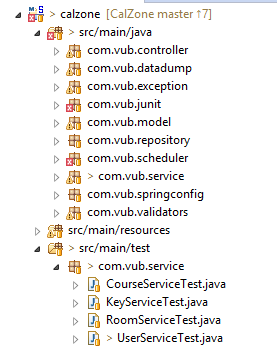
\includegraphics[width=90mm]{img/dir.png}
\caption{Directorystructuur van testbestanden.}
\label{dirstruct}
\end{figure}

\section{Uitgevoerde tests}
In de applicatie worden verschillende tests uitgevoerd. In onderstaande tabel staan alle uitgevoerde tests. Testklasse duidt de klasse aan (.java bestand) in het project waarin de test wordt uitgevoerd, en testnaam is de naam van de test. In een testklasse kunnen meerdere tests bestaan. Onderdeel slaat op het onderdeel van de applicatie waar de test   zich mee bezig houdt - dit wil zeggen opslag van data in de database, testen van regels in de scheduler, enz...

\begin{table}[htbp]
	\centering
	\caption{Tests in de applicatie}
	\begin{tabularx}{\textwidth}{|X|X|X|X|}
	    \hline
		\textbf{Testklasse} & \textbf{Testnaam} & \textbf{Onderdeel} & \textbf{Beschrijving} \\ \hline
		CourseServiceTest	& testCourseCreation & Database & Test het aanmaken van een Course in de database (correcte opslag van velden) \\ \hline
		KeyServicetest & testKeyCreation & Database & Tests m.b.t. aanmaken van keys in de database \\ \hline
		RoomServiceTest & testRoomCreation & Database & Test of een lokaal kan aangemaakt worden in de database \\ \hline
		UserServiceTest & testUserCreation & Database & Test of een user kan aangemaakt worden in de database \\ \hline
		UserServiceTest & testUserActivation & Activatie & Test of users successvol geactiveerd kunnen worden (alleen met een activatie-key) \\ \hline
		EmailValidatorTest & notRealEmail & Validatie & Test of foute e-mailadressen niet geaccepteerd worden \\ \hline
		EmailValidatorTest & notRealEmail2 & Validatie & Andere test op foute-email adressen \\ \hline
		EmailValidatorTest & realEmail & Validatie & Test of een echt e-mail wordt geaccepteerd \\ \hline
		SchedularTest & schedulingRangeTest & Schedular & 4 vakken moeten gescheduled worden in veel tijdslots met één lokaal \\ \hline
		
	\end{tabularx}
\end{table}

\newpage
\section{Belangrijkste Java code conventies}
Ook bij het testen van de applicatie moeten de Java conventies gehanteerd worden. 
Hieronder staan de belangrijkste.
\subsection{Naming conventions}
	\subsubsection{Klassen \& interfaces}
		Gebruik simpele, maar beschrijvende namen (zelfstandige naamwoorden) die iets zeggen over de klasse. Elk zelfstandig woord in de klassenaam begint met een hoofdletter. Vermijd acroniemen, tenzij deze algemeen gebruikt worden (zoals URL en HTTP).
		\\ \\
		\emph{\textbf{class Course;}} \\
		\emph{\textbf{class ProfilePageController;}}
		
	\subsubsection{Methoden}
		Namen van methoden beginnen met werkwoord (en een lowercase letter), met hoofdletters voor elk volgend woord.
		Merk ook op dat in het geval van booleaanse waarden, de getters en setters steeds beginnen met is, bijvoorbeeld \emph{isProjectorEquipped} (m.b.t. projectors in een lokaal). 
		Dit in tegenstelling to het foute \emph{hasProjector}.
		\\ \\
		\emph{\textbf{run();}} \\
		\emph{\textbf{runTests();}} \\
		\emph{\textbf{runTestInBackground();}}
		
	\subsubsection{Variabelen}
		Variabelen beginnen met een lowercase letter, met opeenvolgende woorden gestart worden met een hoofdletter. 
		De naam van een variabele moet kort, maar toch beschrijvend zijn. 
		De namen van constante variabelen in een klasse zijn volledig uppercase, met opeenvolgende woorden gescheiden door een underscore.
		\\ \\		
		\emph{\textbf{float width;}} \\
		\emph{\textbf{float minWidth;}} \\
		\emph{\textbf{int MIN\_WIDTH $=$ 1;}} \\
		\emph{\textbf{boolean DEBUG $=$ false;}} \\
		
		Bovendien wordt ook één declaratie per lijn aangemoedigd, omdat dit het schrijven van commentaar kan aanmoedigen.
		\\ \\
		\emph{\textbf{float width, height;} // fout} \\
		\emph{\textbf{float width;} // Width of the bridge} \\
		\emph{\textbf{float height;} // Height of the bridge}
		

\subsection{Klasse en interface declaraties}
	\begin{itemize}
		\item{Bij aanroep van een methode, geen spatie tussen de methode naam en het openende haakje}
		\item{De open brace \"\{\" staat op dezelfde lijn als de naam van de declaratie}
		\item{De sluitende brace staat automatisch op een nieuwe regel, tenzij de methode een lege body heeft}
		\item{Methoden zijn gescheiden door een blanke regel}
	\end{itemize}
